In this chapter you will learn how to make your
own sourdough starter. Before doing so you will
quickly learn about baker's math. Don't worry,
it's a very simple way how to write recipe in
a cleaner more scalable way. Once you get the hang
of it you will want to write every recipe this way.
You will learn to understand the signs to determine
your starter's readiness.  Furthermore you will
also learn how to store your starter for
long-term storage.

\section{Baker's math}
\label{section:bakers-math}

In a large bakery a determining factor is how
much flour you have at hand. Based on the amount
of flour you have you can calculate how many
breads or buns you can make. To make it easy
for bakers the quantity of each ingredient
is calculated as a percentage based on how much flour you have.
Let me demonstrate this with a small example from
a pizzeria.  In the morning you check and you realize you
have around 1 kilogram of flour.
Your default recipe calls for around 600 grams of water.
That would be a typical pizza dough, not too dry but
also not too wet. Then you would be using around 20 grams
of salt and around 100 grams of sourdough starter.
\footnote{This is my go to pizza dough recipe. In Napoli
modern pizzerias would use fresh or dry yeast. However
traditionally pizza has always been made with sourdough.}
The next day you suddenly have 1.4 kilograms of flour
at hand and thus can make more pizza dough. What do you do?
Do you multiply all the ingredients by 1.4? Yes you could,
but there is an easier way. This is where baker's math
comes in handy. Let's look at the default recipe with baker's
math and then adjust it for the 1.4 kilogram flour quantity.

\begin{table}[H]
\centering
\resizebox{\textwidth}{!}{%
\begin{tabular}{|l|r|r|}
\hline
\textbf{Ingredient}    & \multicolumn{1}{l|}{\textbf{Explanation}} & \multicolumn{1}{l|}{\textbf{Explanation}}  \\ \hline
1000g flour            & 100\%                                     & 1000g of 1000g = 100\%                     \\ \hline
600g water             & 60\%                                      & 600g of 1000g = 60\%                       \\ \hline
100g sourdough starter & 10\%                                      & 100g of 1000g = 10\%                       \\ \hline
20g salt               & 2\%                                       & 20g of 1000g = 2\%                         \\ \hline
\end{tabular}%
}
\end{table}

Note how each of the ingredients is calculated as a percentage
based on the flour. The 100 percent is the baseline as the absolute
amount of flour that you have at hand. In this case that's 1000 grams
(1 kilogram).

Now let's go back to our example and just the flour as we have
more flour available the next day. As mentioned the next day
we have 1.4 kilograms at hand (1400 grams).

\begin{table}[H]
\centering
\resizebox{\textwidth}{!}{%
\begin{tabular}{|l|r|r|}
\hline
\textbf{Ingredient} & \multicolumn{1}{l|}{\textbf{Baker's math}} & \multicolumn{1}{l|}{\textbf{Calculated value}} \\ \hline
Flour               & 100\%                                      & 1400*1 = 1400g                                 \\ \hline
Water               & 60\%                                       & 1400*0.6 = 840g                                \\ \hline
Sourdough starter   & 10\%                                       & 1400*0.1 = 140g                                \\ \hline
Salt                & 2\%                                        & 1400*0.02 = 28g                                \\ \hline
\end{tabular}%
}
\end{table}

For each ingredient we calculate the percentage
based on the flour available (1400 grams.) So for the water
we calculate 60 percent based on 1400. Open up your
calculator and type in 1400 * 0.6 and you have
the absolute value in grams that you should be using.
In that case that is 840 grams. Proceed and do the same
thing for all the other ingredients and you know
your recipe.

Let's say you would want to use 50 kilograms of flour
the next day. What would you do? You would simply proceed
and calculate the percentages one more time. I like this
way of writing recipes a lot. Imagine you wanted to make
some pasta. You would like to know how much sauce you should
be making. Now rather than making a recipe just for you, the
hungry family arrives. You are tasked with making pasta
for 20 people. How would you calculate the amount of sauce
you need? You go to the internet and check a recipe and then
are completely lost when trying to scale it up.

\section{The process of making a starter}

\begin{figure}[!htb]
  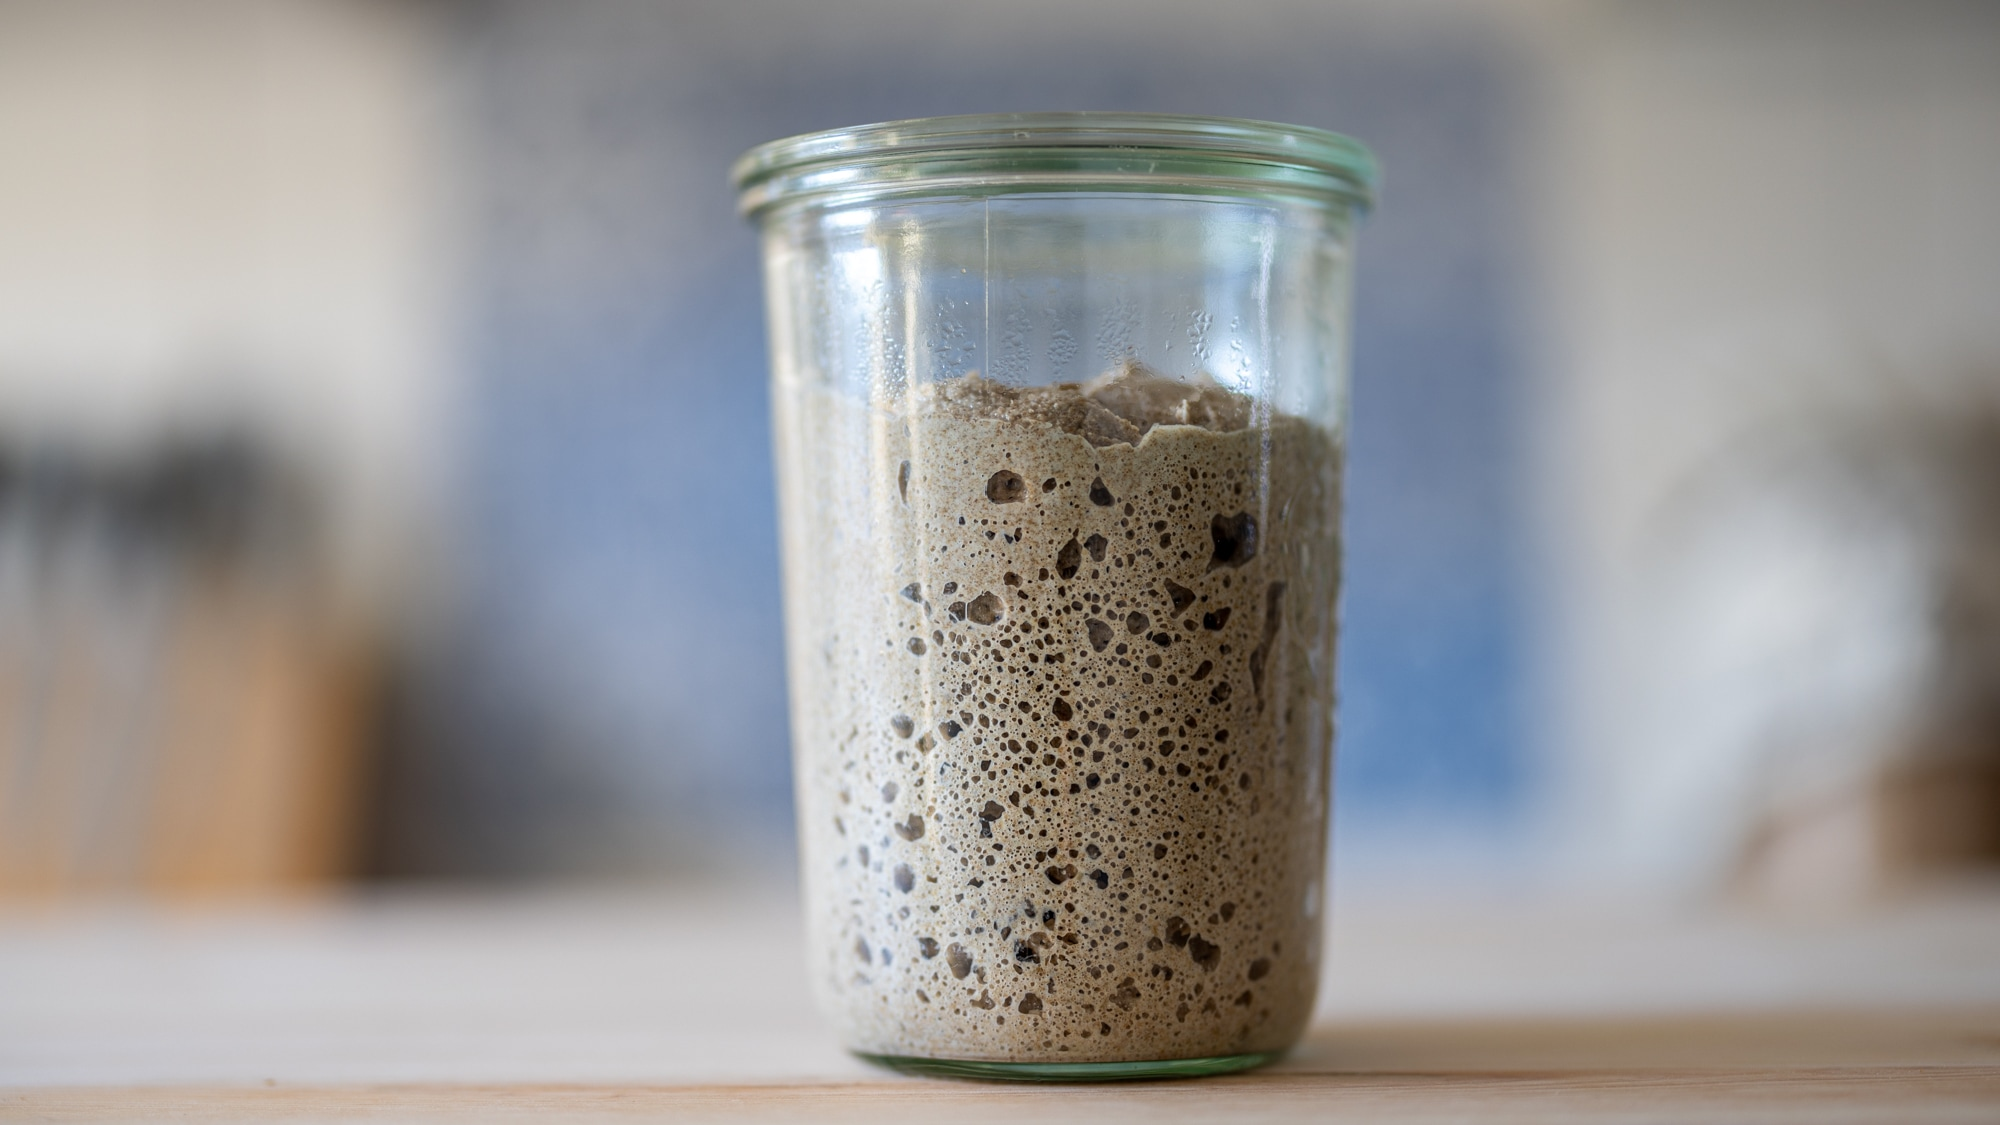
\includegraphics[width=\textwidth]{sourdough-starter.jpg}
  \caption{A very active sourdough starter shown by the bubbles in the dough}
  \label{fig:sourdough-starter}
\end{figure}

Making a sourdough starter is very easy. All you need
is a little bit of patience. The flour you should
use to setup your starter is ideally a whole flour.
You could use whole wheat, whole rye, whole spelt or
any other flour you have. In fact gluten free flours such
as rice or corn would also work. Don't worry, you can
change the flour later. Use whatever whole flour you
already have at hand.

Your flour is contaminated with millions of microbes. As explained
before in the chapter about wild yeast and bacteria, these
microbes live on the surface of the plant. That's why
a whole flour works better because you have more natural
contamination of the microbes you are trying to cultivate
in your starter. More of them live on the hull compared to the
endophytes living in the grain.

Simply weigh around 50 grams of flour and add another 50
grams of water. It doesn't have to be exactly 50 grams of both
water or flour. You could also be using less and/or simply eyeball
it. The values are just shown as a reference. Don't use chlorinated
water to setup your starter. It should be bottled water ideally,
or here in Germany we can just use our tap water. The hydration
of your dough is 100 percent. This means you have equal parts
of flour and water. Stir everything together so that all the flour
is properly hydrated. By adding water many of your microbe's
spores become activated. They exit hibernation mode and
become alive again. Cover your mixture with a lid. I like to
use a glas and place another inverted one on top. The container shouldn't
be airtight. You still want some gas exchange to be possible.

\begin{figure}[!htb]
  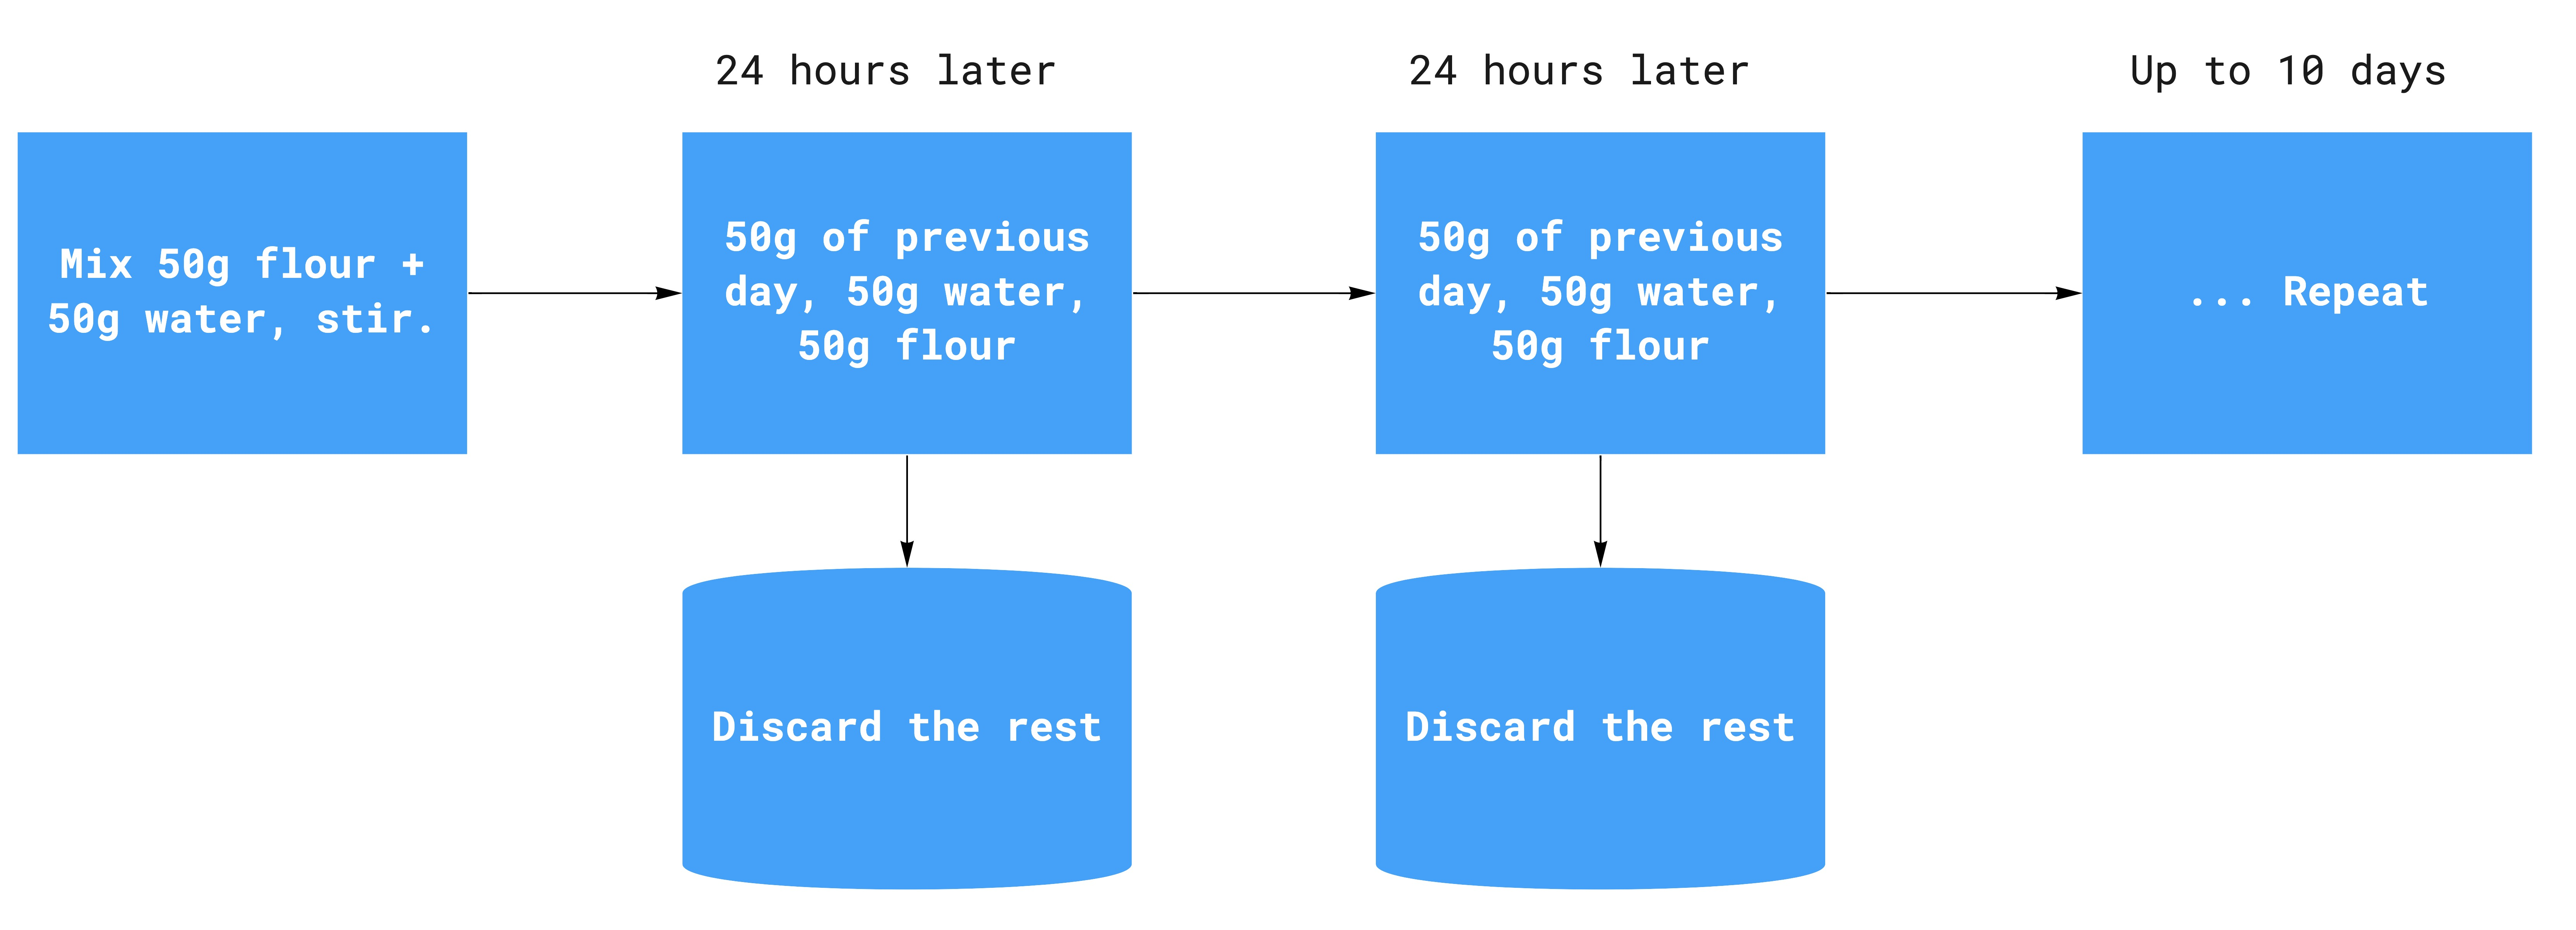
\includegraphics[width=\textwidth]{sourdough-starter-process.jpg}
  \caption{The process of making a sourdough starter from scratch}
  \label{fig:sourdough-starter-process}
\end{figure}

Now an epic battle starts to begin. In one study scientists
have identified more than 150 different yeast species living
on a single leaf of a plant \cite{yeasts+biocontrol+agent}.
All of the different yeasts and bacteria are trying to get
the upper hand in this battle. Other pathogens such as mold
are also being activated as we added water. Only the strongest
most adapt microorganisms will survive. By adding water to the
flour the starches start to degrade. The seedling tries to
sprout but it no longer can. Essential for this process is the
amylase enzyme. The compact starch is broken down to more
digestible sugars to fuel plant growth. Glucose is what the
plant needs in order to grow. The microorganisms that survive
this frenzy are adapt to consuming glucose. Luckily for us
bakers the yeast and bacteria know very well how to metabolize
glucose. This is what they have been fed in the wild by the plants.
By forming patches on the leaf and protecting the plant from
pathogens they received glucose in return for their services.
Each of the microbes tries to defeat the other by consuming the
food fastest, producing agents to inhibit food uptake or by producing
bactericides and/or fungicides. This early stage of the starter
is very interesting as more research could possibly reveal
new fungicides or antibiotics. Depending on where your flour
is from the starting microbes of your starter might be different
than the ones from another starter. Some people have also reported
how the microbes from your hand or air can influence your starter's
microorganisms. This makes sense to a certain extent. Your
hand's microbes might be good at fermenting your sweat, but
probably not so good and metabolizing glucose. The contamination
of your hands or air might play a minor role in the initial epic
battle. But only the fittest microbes fitting the sourdough's
niche are going to survive. This means the microorganisms that know
how to convert maltose or glucose will have the upper hand. Or these
microbes that ferment the waste of the other microbes. Ethanol created
by the yeast is metabolized by the bacteria in your sourdough. That's
why a sourdough has no alcohol. I can confirm the role of aerial
contamination to a certain extent. When setting up a new sourdough
starter the whole process is quite quick for me. After a few
days my new starter seems to be quite alive already. This might
be due to previous contamination of flour fermenting microbes in
my kitchen.

Wait for around 24 hours and observe what happens to your starter.
You might see some early signs of fermentation already. Use your nose
to smell the dough. Look for bubbles in the dough. Your dough
might already have increased in size a little bit. Whatever
you see and notice is a sign of the first battle. Some microbes
have already been outperformed. Others have won the first battle.
After around 24 hours most of the starch has been broken down
and your microbes are hungry for additional sugars. With a spoon
take around 10 grams from the previous day mixture and place
it in a new container. Again - you could also simply eye ball
all the quantities. It does not matter that much. Mix the 10
grams from the previous day with another 50 grams of flour
and 50 grams of water. Note the ratio of 1:5. I very often use
1 part of old culture with 5 parts of flour and 5 parts of water.
This is also very often the same ratio I use when making a dough.
A dough is nothing else than a sourdough starter with slightly different
properties. I'd always be using around 100-200 grams of starter
for around 1000 grams of flour (baker's math: 10-20 percent).
Homogenize your new mixture again with a spoon. Then cover
the mix again with a glas or a lid. If you notice the top of
your mixture dries out a lot consider using another cover. The
dried out parts will be composted by more adapt microbes such as
mold. In many user reports I saw mold being able to damage
the starter when the starter itself dried out a lot. You will
still have some mixture left from your first day. As this contains
possibly dangerous pathogens that have been activated we will discard
this mixture for now. Once your sourdough starter is mature never
discard it. It's long fermented flour that is an excellent addon
used to make crackers, pancakes and or delicious hearty sandwich
breads. I also frequently dry it and use it as a rolling agent
for pizzas that I am making.

You should hopefully again see some bubbles, the starter increasing
in size and/or the starter changing its smell. Some people give
up after the second or third day. That is because the signs might no longer
be as dominant as they were on day one. The reason for this lies in only a few
select microbes starting to take over the whole sourdough starter. The most
adapt ones are going to win. They are very small in quantity and will
grow in population with each subsequent feeding. Even if you see no signs
of activity directly, don't worry. There is activity in
your starter on a microscopic level.

24 hours later again we will repeat the same thing again until
we see that our sourdough starter is active. More on that in the
next section of this book.

\section{Determining starter readiness}

For some people the whole process of setting up a starter takes
only 4 days. For others it can take 7 days, for some even 20 days.
This depends on several factors including how good your wild microbes
are fermenting flour. Generally speaking with each feeding
your starter becomes more adapt to its environment. Your
starter will become better at fermenting flour. That's why
a very old and mature starter you receive from a friend might
be stronger than your own starter initially. Over time
your sourdough starter will catch up. Similarly modern baking
yeast has been isolated like this from century old sourdough
starters.

\begin{figure}[!htb]
  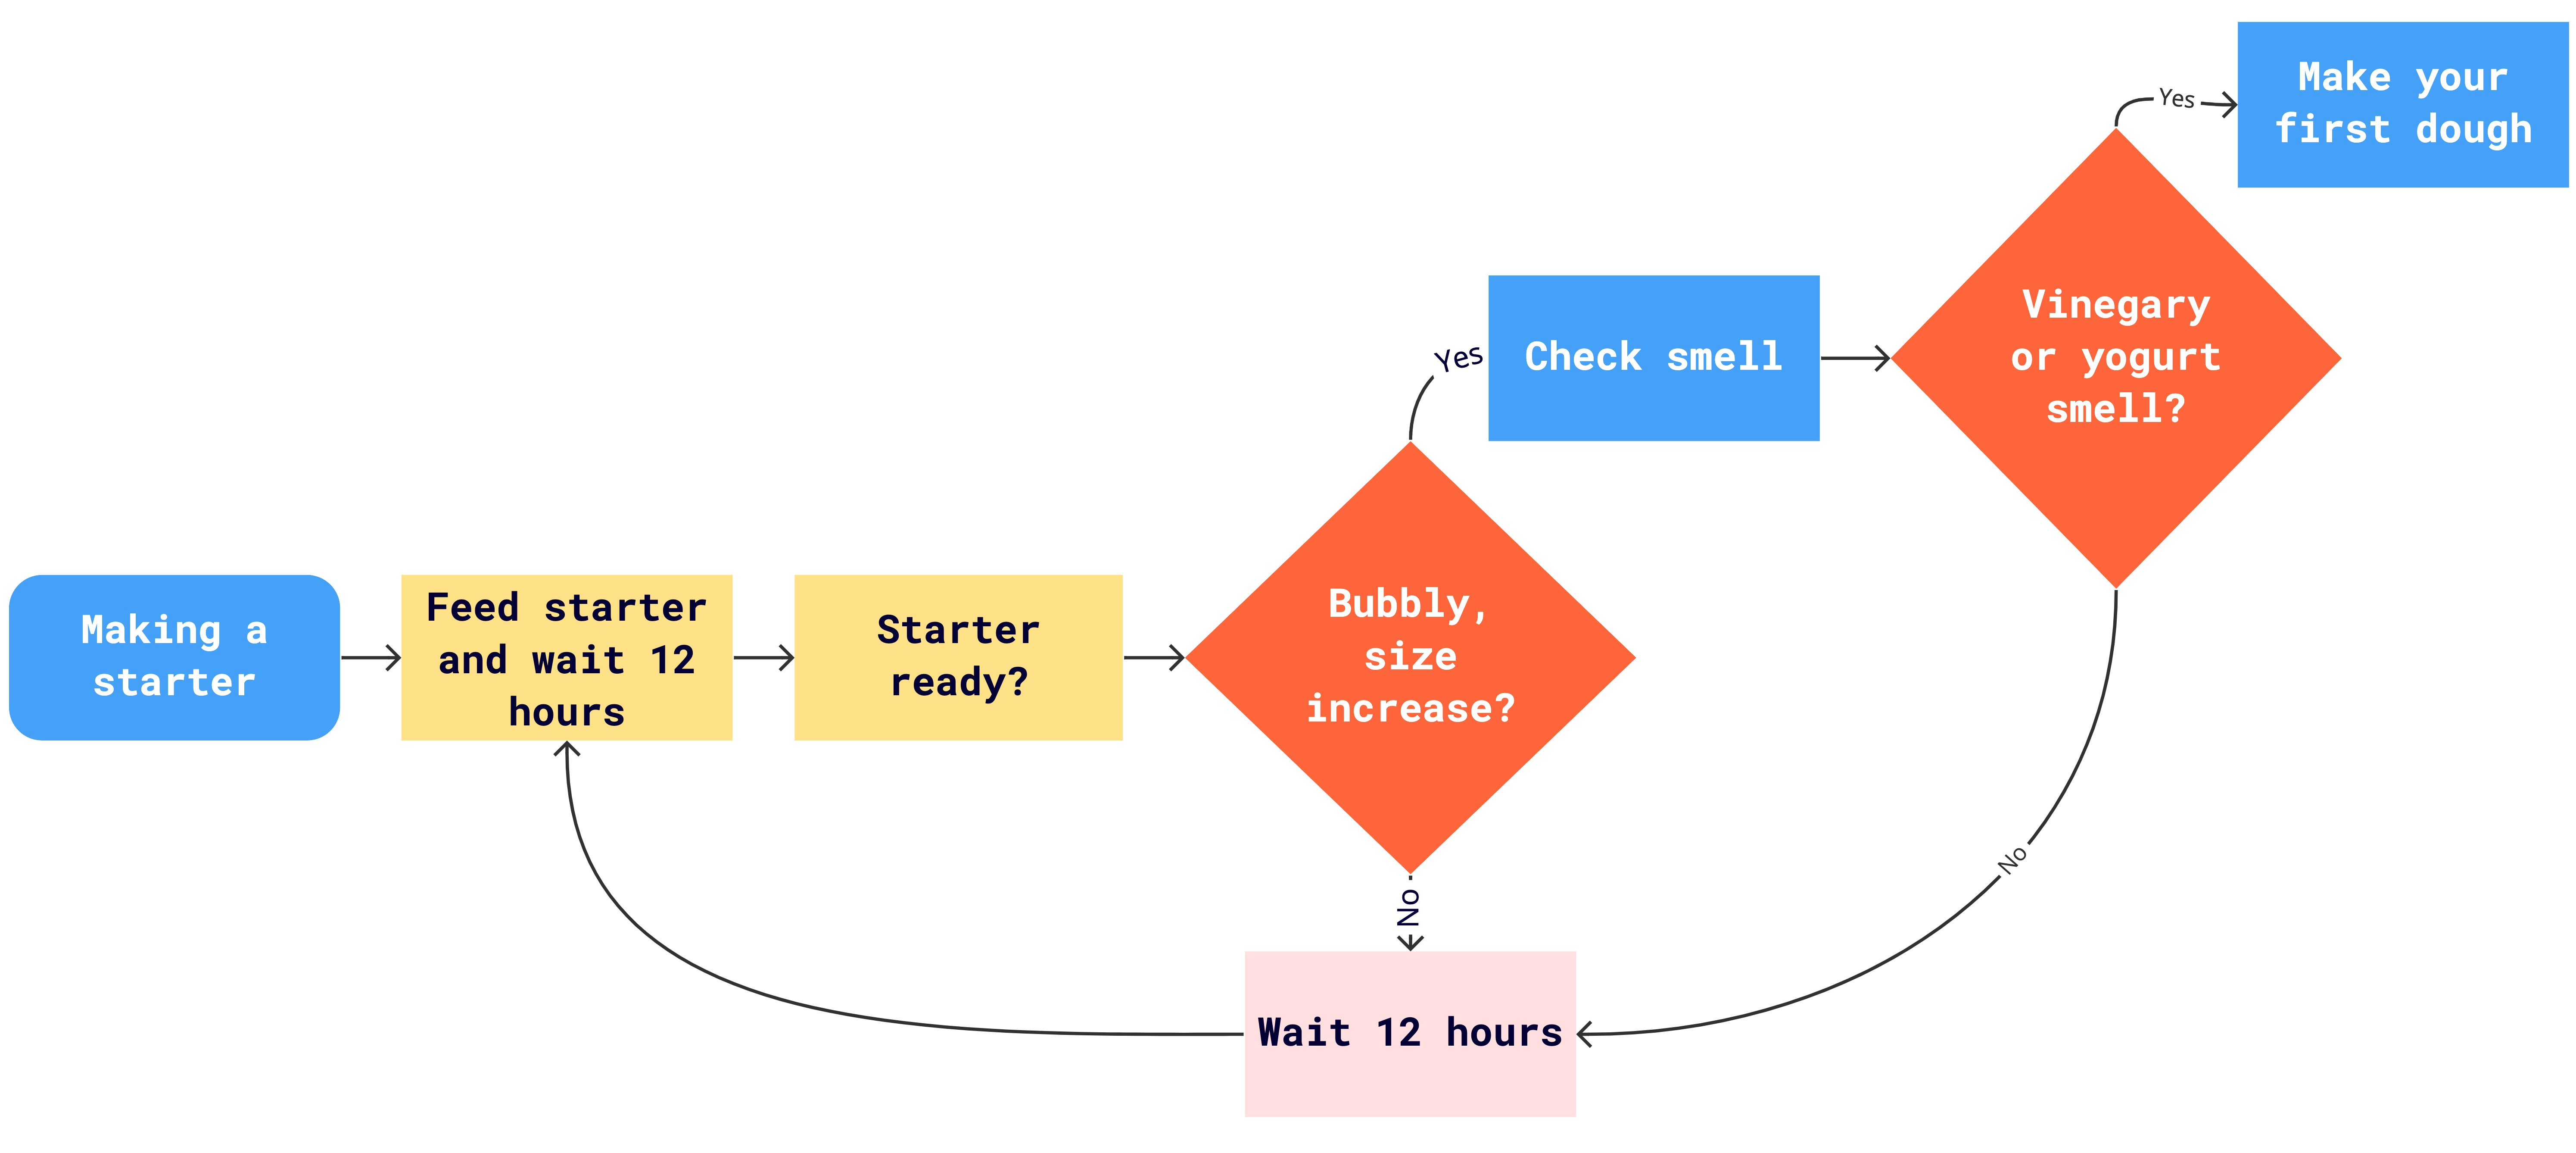
\includegraphics[width=\textwidth]{sourdough-starter-readiness.jpg}
  \caption{A flowchart showing how to check if your sourdough starter is ready
  to be used}
  \label{fig:sourdough-starter-readiness}
\end{figure}

The key signs to look at are bubbles that you see in your starter
jar. This is a sign that the yeast is metabolizing your
dough and creates CO2. The CO2 is trapped in your dough
matrix and then visualized on the edges of the container.
Also note the size increase of your dough. The amount of size
is irrelevant. Some bakers claim it doubles, triples or quadruples.
The amount of size increase depends on your microbes, but also on
the flour that you using to make the starter. A wheat flour contains
more gluten and will thus result in a higher size increase. At
the same time the microbes are probably not more active compared
to when living in a rye sourdough. You could only argue that
wheat microbes might be better at breaking down gluten compared
to rye microbes. That's one of the reasons why I decided to change
the flour of my sourdough starter quite often. I had hoped to create
an all-round starter that can ferment all sorts different flour.\footnote
{Whether this is actually working I can't scientifically say.
Typically the microbes that have once taken place are very strong
and won't allow other microbes to enter. My starter has initially
been made with rye flour. So chances are that the majority of
my microorganisms are from a rye source.} Your nose is also
a great tool to determine starter readiness. Depending on
your starter's microbiome you should notice either the smell
of lactic acid or acetic acid. Lactic acid has dairy yogurty notes.
The acetic acid has very strong pungent vinegary notes. Some
describe the smell as glue or acetone. Combining the visual clues
of size increase and pockets plus the smell is the best way
to determine starter readiness.

In rare events your flour might be treated and prevent microbe growth.
This can happen if the flour is not organic and a lot of biochemical
agents have been used by the farmer. In that case simply try again
with different flour. 7 days is a good period of time to wait before
trying again.

Another methodology used by some bakers is the so called \emph{float test}.
The idea is to take a piece of your sourdough starter and place it
on top of some water. If the dough is full with gas it will float
on top of the water. If it's not ready it can't float and will
sink to the bottom of the glas. This test does not work with every flour.
Rye flour for instance can't retain the gas as well as wheat flour
and thus in some cases will not float. That's why I personally
don't use this test and can't recommend it.

Once you see your starter is ready I would recommend to give it
one last feeding and then you are ready to make your dough in the
evening or the next day. For the instructions to make your
first dough please refer to the next chapters in this book.

If your first bread failed chances are your fermentation hasn't
worked as expected. In many cases the source is your sourdough starter. Maybe
the balance of bacteria and yeast hasn't been optimal yet. In that case a good
solution is to keep feeding your starter once per day. With each feeding your
starter becomes better at fermenting flour. The microbes will adapt more and
more to the environment. Please also consider reading the stiff sourdough starter
chapter in this book. The stiff sourdough starter helps to boost the
yeast part of your sourdough and balance the fermentation.

\section{Maintenance}

\begin{figure}[!htb]
  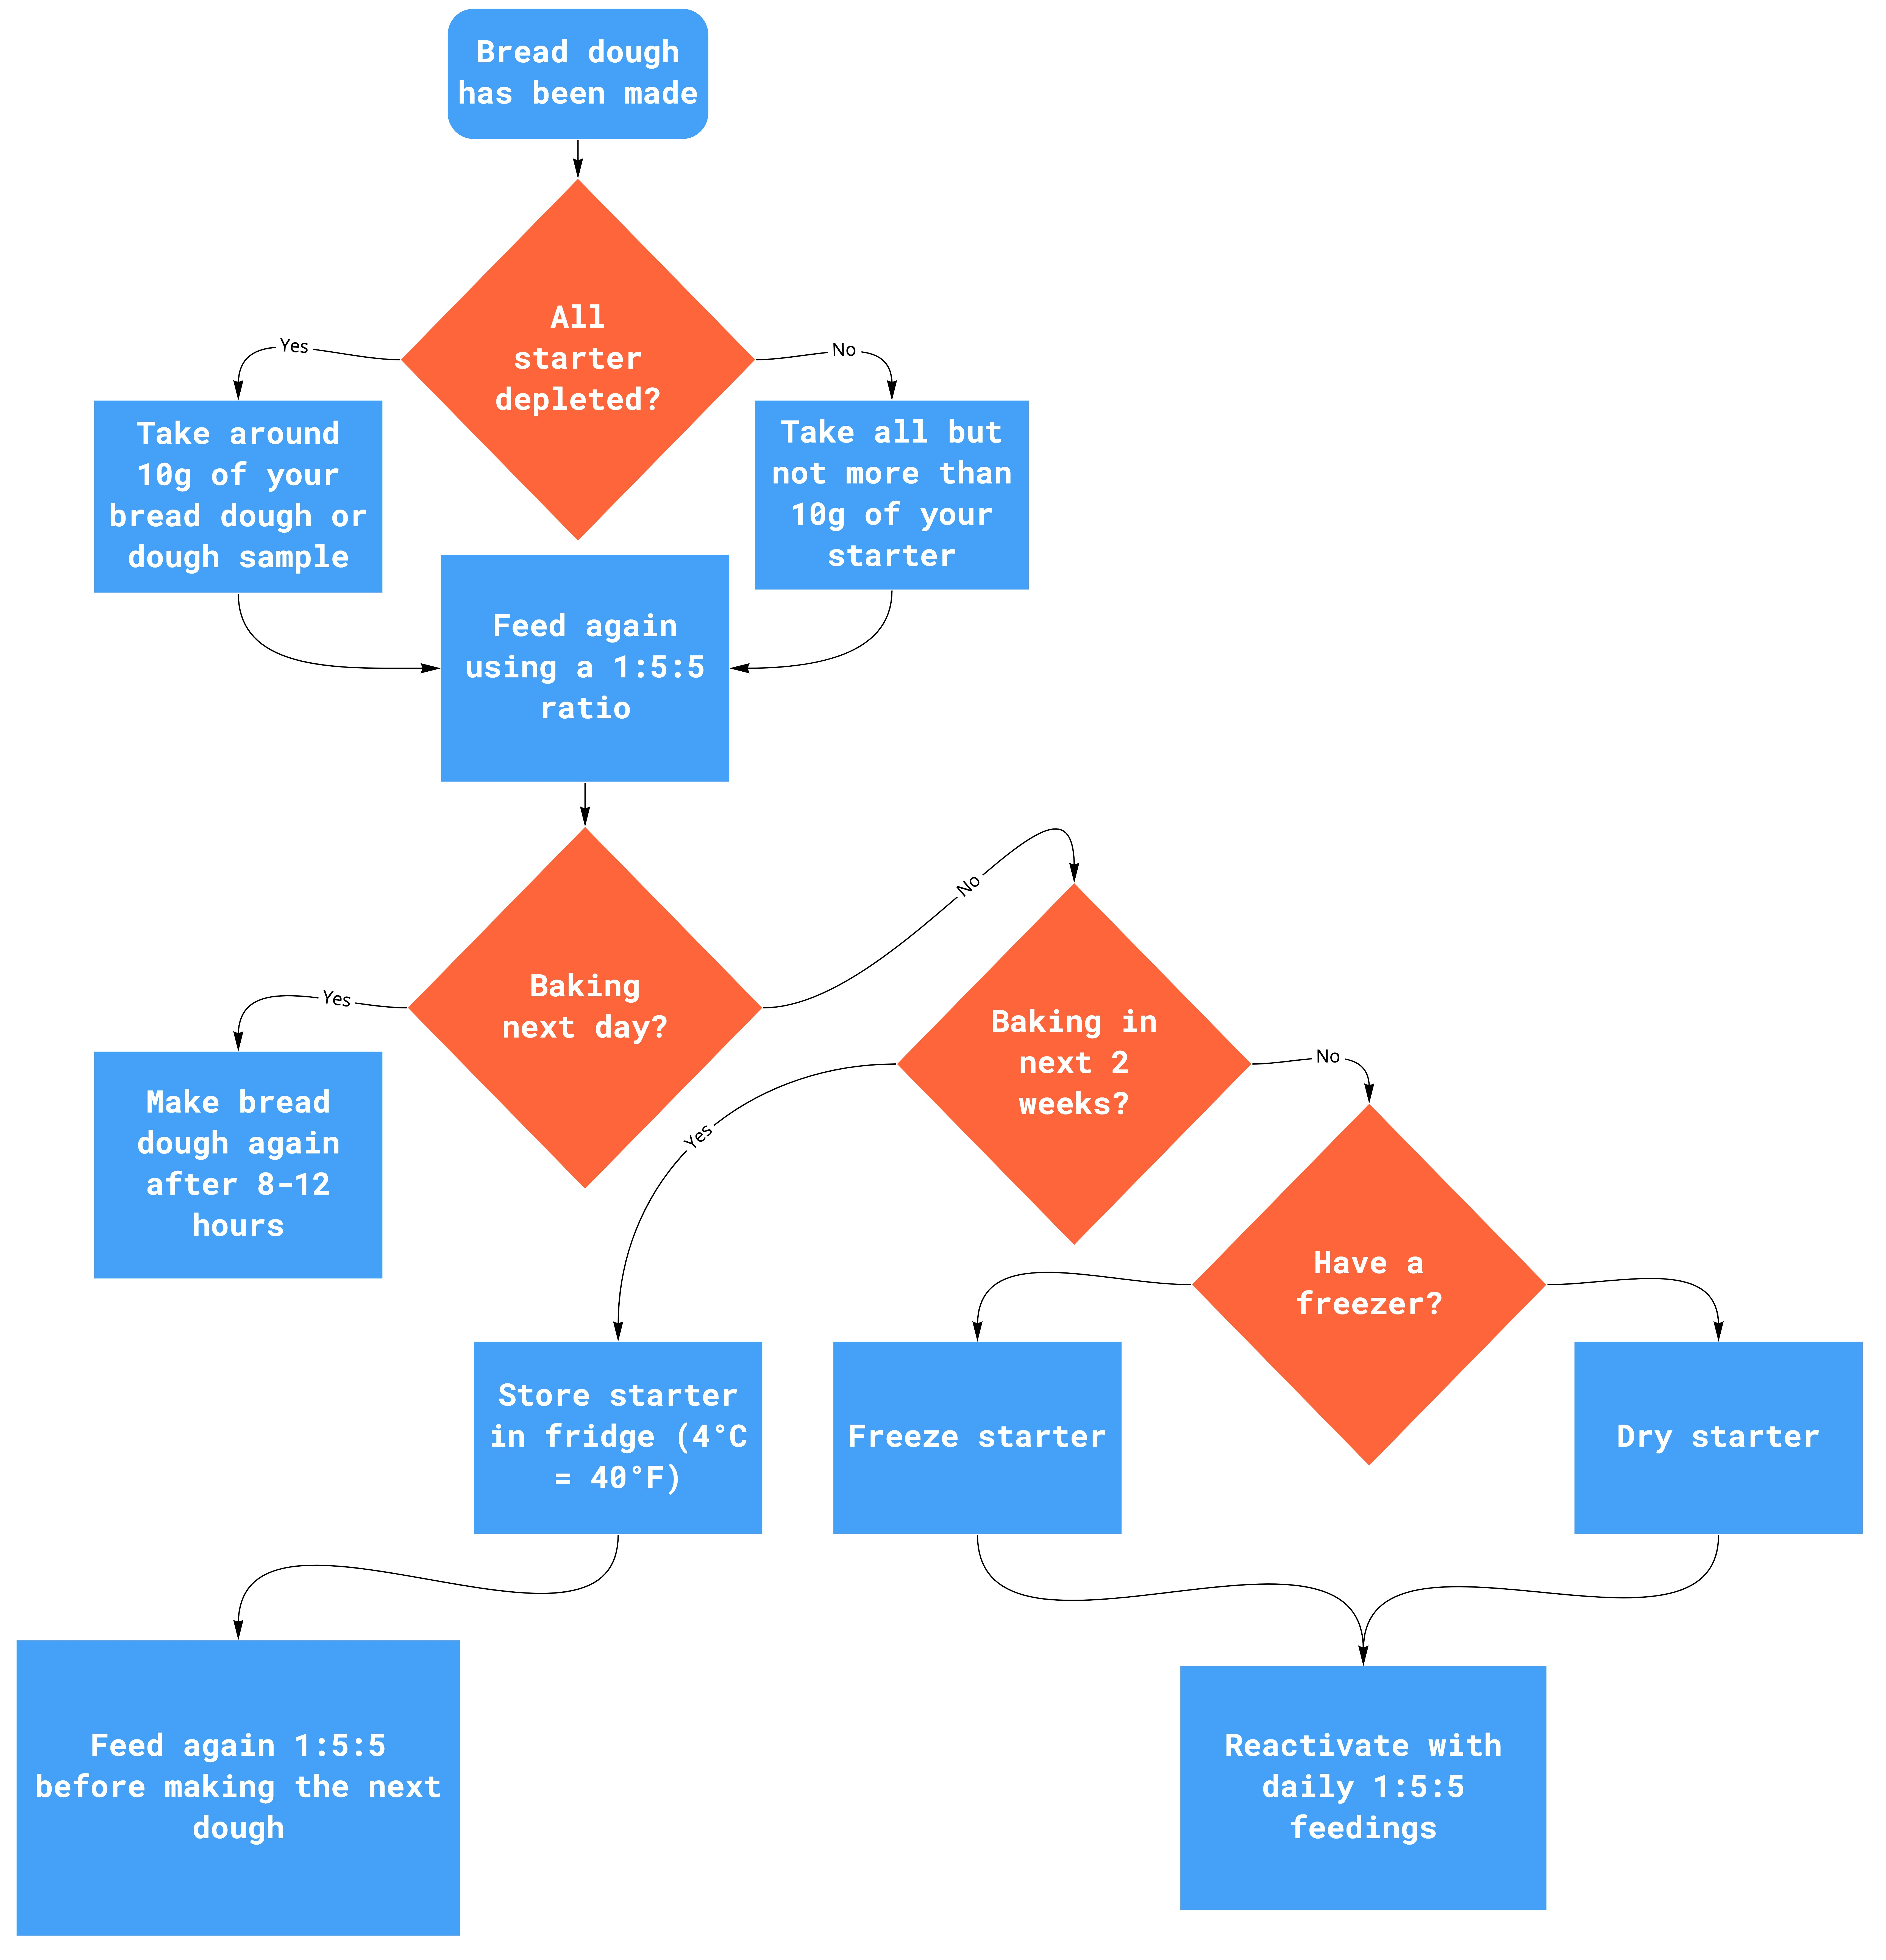
\includegraphics[width=\textwidth]{sourdough-starter-maintenance-process.jpg}
  \caption{A full flowchart showing how to conduct proper starter maintenance}
  \label{fig:sourdough-maintenance-process}
\end{figure}

You have made your sourdough starter and your first bread. How do you perform
maintenance for your starter? There are countless of different maintenance
methods out there. Some people go completely crazy about their starter and
perform daily feedings of the starter. The key to understanding how properly
conduct maintenance is to understand what happens to your starter after you
used it to make a dough. Whatever starter you have left, or a tiny piece of
your bread dough can serve to make your next starter.\footnote{I very often use all my
starter to make a dough. So if the recipe calls for 50g of starter I make
exactly 50g starter in advance. This means I have no starter left. In that
case I would proceed to take tiny bit of the dough at the end of the
fermentation period. This piece I would use to regrow my starter again}


As explained earlier your starter is adapt
to fermenting flour. The microbes in your starter are very resilient. They
block external pathogens and other microbes. That is the reason why when
buying a sourdough starter you will preserve the original microbes. They are
likely not going to change in your starter. They are outcompeting other
microbes when it comes to fermenting flour. Normally everything in nature
starts to decompose after a while. However the microbes of your starter have
very strong defense mechanisms. In the end your sourdough starter can be
compared to pickled food. Pickled food has been shown to stay good for a very
long period of time \cite{pickled+foods+expiration}. The acidity of your sourdough starter is quite
toxic to other microbes. The yeast and bacteria though have adapted to living
in the high acid environment. Compare this to your stomach, the acidity
neutralizes many possible pathogens. As long as your starter has sufficient
food available it will outcompete other microbes. When the starter runs out of
food the microbes will start to sporulate. They prepare for a period of no
food and will then reactivate the moment new food is present. The
spores are very resilient and can survive under extreme conditions.
Scientists have claimed they found 250 million year old spores still active
spores \cite{old+spores}. While being spores
they are however more vulnerable to external pathogens such as mold.
Everything in nature is at some point decomposed and broken down by other
microorganisms. Under ideal conditions though the spores can survive for a
long time.

But as long as they stay in the environment of your starter they live
in a very protected protected environment. Other fungi and bacteria have a hard time decomposing your left over starter mass.
I have seen only very few cases where the starter actually died. It is almost impossible
to kill a starter.

What happens though is that the balance of yeast and
bacteria changes in your starter. The bacteria is more adapt to living
in the acidic environment. This is a problem when you make another dough.
You want to have the proper balance of fluffiness and sour notes.
When a starter has hibernated for a long period
of time chances are that you do not have a desirable balance of microbes.
Furthermore depending on the time your starter hibernated you might only have
sporulated microbes left. So a couple of feedings will help to get your
sourdough starter into the right shape again.

The following are a couple of scenarios that help you to conduct proper
starter maintenance, depending on when you want to bake the next time.

\textbf{I would like to bake again the next day:}

Simply take whatever starter you have left and feed it again. If you depleted
all your starter you can cut a piece of your dough. The dough itself is
nothing different than a gigantic starter. I recommend a 1:5:5 ratio like
mentioned before. So take 1 piece of starter, feed with 5 parts of flour and 5
parts of water. If it is very hot where you live, or if you want to make the
bread around 24 hours later after your last feeding, change the ratio. In that
case I would go for a 1:10:10 ratio. Sometimes I don't have enough starter.
Then I even use a ratio of 1:50:50 or 1:100:100. Depending on how much new
flour you feed it takes longer for your starter to be ready again.

\textbf{I would like to take a break and bake next week:}

Simply take your leftover starter and place it inside of your fridge. It will stay good
for a very long period of time. The only thing I see happening is the surface
drying out in the fridge. So I recommend to drown the starter in a little bit
of water. This extra layer of water provides a good protection from the top
part drying out. As mold is aerobic it can not grow efficiently grow under
water \cite{mold+anaerobic}. Before using the starter again simply either stir
the liquid into the dough or drain it. If you drain the liquid you can use it
to make a lacto fermented hot sauce for instance.

The colder it is the longer you preserve a good balance of yeast and
bacteria. Generally the warmer it is the faster the fermentation process is.
The colder the slower the whole process becomes.
Below 4°C the starter fermentation comes to a complete halt.

\textbf{I would like to take a several months break:}

Drying your starter might be the best option to preserve it in this case. As
you remove humidity and food your microbes will sporulate. As there is no
humidity the spores can resist other pathogens very well. A dried starter can
be good for years.

Simply take your starter and mix it with flour. Try to crumble the starter as
much as possible. Add more flour continuously until you notice that the is no
moisture left. Place the flour starter at a dry place in your house. Let it
dry even more. If you have a dehumidifier you can use this to speed up the
process. Set it to around 30°C and dry the starter for 12-20 hours. The next
day return your starter. It is in a vulnerable state as there is still a bit
of humidity left. Add some more flour to speed up the drying process. Repeat
for another 2 days until you feel that there is no humidity left. This is
important or else it might start to mold. Once this is done simply store the
starter in an airtight container. If you can proceed and freeze
the dried starter. Both options work perfectly fine. Your sporulated starter
is now waiting for your next feeding.

Initially it would take 3 days or so for my starter to become alive again
after drying and reactivating it. If I do the same thing now my starter is
sometimes ready after a single feeding. It seems that the microbes adapt. The ones
that survive this shock become dominant subsequently.

So in conclusion the maintenance mode you choose depends on when you want to bake next.
The goal of each new feeding is to make sure your starter
has a desired balance of yeast and bacteria when making a dough. There is no need to provide your
starter with daily feedings, unless it is not mature yet. In that case each
subsequent feeding will help to to make your starter more adapt at fermenting
flour.
